%\documentclass[conference]{IEEEtran}
\documentclass[10pt, conference, letterpaper]{IEEEtran}
%% INFOCOM 2013 addition:
\makeatletter
\def\ps@headings{%
\def\@oddhead{\mbox{}\scriptsize\rightmark \hfil \thepage}%
\def\@evenhead{\scriptsize\thepage \hfil \leftmark\mbox{}}%
\def\@oddfoot{}%
\def\@evenfoot{}}
\makeatother
\pagestyle{headings}

\usepackage{amsmath}
\usepackage{algorithm}
\usepackage{algorithmic}
\usepackage{graphicx}
\usepackage{cite}
%\usepackage{mathrsfs}
\usepackage[bookmarks=false]{hyperref}
\usepackage{array}
\usepackage{cases}
\usepackage{booktabs}
\usepackage{multirow}
\usepackage{threeparttable}
\usepackage{epstopdf}


%
%\begin{flushleft}\fontsize{8.5pt}{0.6\baselineskip}\selectfont{Remarks: 1) ``$-$" means the algorithm is not applicable to
%oblivious blind rendezvous; 2) ETTR means expected time to rendezvous (note: MMC cannot guarantee rendezvous in bounded time); 3) $P$ is the smallest prime number larger than $N$, $P=O(N)$. 4) $k_a$ and $k_b$ denote the numbers of two users' available channels; 5) SCH in this paper is only suitable for synchronous users.
%}\end{flushleft}


\newtheorem{property}{Property}[section]
\newtheorem{theorem}{Theorem}
\newtheorem{lemma}{Lemma}[section]
\newtheorem{claim}[lemma]{Claim}
\newtheorem{remark}{Remark}[section]
\newtheorem{definition}{Definition}[section]
\newtheorem{corollary}{Corollary}
\newtheorem{problem}{Problem}

\ifCLASSINFOpdf

\else

\fi

\ifCLASSOPTIONcompsoc
\usepackage[tight,normalsize,sf,SF]{subfigure}
\else
\usepackage[tight,footnotesize]{subfigure}
\fi

% correct bad hyphenation here
\hyphenation{op-tical net-works semi-conduc-tor}


\begin{document}




\title{How Local Information Improves Rendezvous in Cognitive Radio Networks}

%\author{\IEEEauthorblockN{
%Zhaoquan Gu\IEEEauthorrefmark{1}, Haosen Pu\IEEEauthorrefmark{1}, Qiang-Sheng Hua\IEEEauthorrefmark{2}, and
%Francis C.M. Lau\IEEEauthorrefmark{3}}
%
%\IEEEauthorblockA{\IEEEauthorrefmark{1}Institute for Interdisciplinary Information Sciences, Tsinghua University,
%Beijing, China\\}
%\IEEEauthorblockA{\IEEEauthorrefmark{2}School of Computer Science $\&$ Technology, Huazhong University of Science and Technology, China\\}
%\IEEEauthorblockA{\IEEEauthorrefmark{3}Department of Computer Science, The University of Hong Kong, Hong Kong, China\\}
%}

\maketitle


\begin{abstract}
Cognitive Radio Network (CRN) is a promising technique aiming at solving the wireless spectrum scarcity problem. Rendezvous is the fundamental process of CRN.  We are devoted to design faster rendezvous algorithms for CRN. We find that local information such as user's ID and the label of an available channel is very useful for designing faster rendezvous algorithms. First, we propose the Sequence-Rotating Rendezvous (SRR) algorithm. SRR algorithm can guarantee rendezvous for any two users $i,j$ in $(2 P^2+2P)$ timeslots, where $P$ is the least prime not less than the total number of channels in the network. SRR algorithm has a lower MTTR than the extant asynchronous anonymous non-oblivious global-sequence-based rendezvous algorithms. Second, we utilize the user's identifier (ID) to design an ID-based Rendezvous (IDR) algorithm. IDR algorithm can guarantee rendezvous for any two users $i$ and $j$ in $(l+1)(P_i+2)(P_j+2)$ timeslots, where $P_i$ and $P_j$ are the smallest primes which are not less than the numbers of available channels of user $i$ and $j$ respectively. IDR algorithm has a lower MTTR than the extant asynchronous non-anonymous oblivious local-sequence-based rendezvous algorithms. Third, we propose a Channel-Label-based Rendezvous (CLR) algorithm which can guarantee rendezvous for any two users in $((P_i +2)(P_j+2) + P_N)(\left \lceil log_2 N \right \rceil + 1)$ timeslots, where $N$ is the overall amount of channels in the network and $P_N$ is the least prime which is not less than $N$.  All of our algorithms can be used in multi-user scenario. We conduct plenty of experiments comparing our algorithms with state-of-the-art rendezvous algorithms under different scenarios, which confirm our analysis.
\end{abstract}


\begin{IEEEkeywords}
Cognitive Radio Network, Local Information, Rendezvous Algorithms, Channel Label, identifier
\end{IEEEkeywords}

\section{Introduction}
Wireless spectrum is an invaluable resource for transmission between wireless devices.
Normally speaking, wireless spectrum is divided into licensed spectrum which is occupied by paying users (also called primary users, PUs) and unlicensed spectrum which is free for unlicensed users (also called secondary users, SUs).
With the development of wireless technology, unlicensed spectrum is becoming more and more severe due to rapid growth of wireless devices \cite{Li2013Economic} and wireless services. However, the utilization rate of licensed spectrum is relatively low \cite{Min2014A} \cite{Jia2010Analysis}. Cognitive radio networks (CRNs) are thus proposed to alleviate the spectrum scarcity problem, which allows SUs to sense and utilize vacant licensed spectrum for communication by equipping with cognitive radios.
\footnote{Unless specifically stated, ``users'' in the rest of the paper refer to SUs.}


In CRN, there exist many important processes such as broadcasting, routing, data gathering, etc. \emph{Rendezvous} is a fundamental process of CRN, which targets finding a licensed channel on which two neighboring users can communicate.
Since PUs have higher priority than SUs, when a PU is occupying a channel, every SU cannot access it.
To construct a communication link on a common channel, some works assume a central controller or a common control channel exists which gets full knowledge of users' available channel sets, then two users can be assigned with a common available channel for communication\cite{Jia2008HC} \cite{Kondareddy2009Cognitive} \cite{Ma2005Dynamic} \cite{Perez2007A}. However, establishing a central controller is cost and vulnerable if a huge number of users require communication concurrently or the central controller gets attacked. Therefore, more distributed rendezvous algorithms are proposed which assume two users do not know each other's information and the users run their algorithms separately  \cite{Lin2013Enhanced} \cite{Gu2013Nearly} \cite{Shin2010A} \cite{Wu2013On} \cite{Wu2014Rendezvous}. This kind of algorithms is also called ``blind'' rendezvous algorithms and it becomes more practical than centralized algorithms. Channel Hopping (CH) technique \cite{Bian2009A} \cite{Bian2011Control} is a widely adopted method in blind rendezvous algorithms, in which a user selects a channel for rendezvous attempt according to a pre-generated channel hopping sequence.
Most blind rendezvous algorithms utilize the labels of channels to construct CH sequences. Some blind rendezvous algorithms also utilize users' IDs in their construction of CH sequences.

\begin{table*}[!t]
\renewcommand{\arraystretch}{1.3}
 \caption{\upshape Comparisons between rendezvous algorithms }
\centering
\begin{tabular}{|c|c|c|c|c|c|c|}
\hline
\multirow{2}*{Algorithm} &  \multirow{2}*{MTTR}  & \multirow{2}*{Time} & Anonymous or & Oblivious or &\multirow{2}*{Sequence} &Symmetric or\\
 &   & & Non-Anonymous & Non-Oblivious & & Asymmetric\\
 \hline
%JS & 3NP(P-G) +3P  & Asynchronous & Anonymous & Non-Oblivious & Global & Single-radio\\
%\hline
DRDS \cite{Gu2013Nearly}& $3P^2 + 2P$  & Asynchronous & Anonymous & Non-Oblivious & Global & Asymmetric\\
\hline
CBH \cite{Gu2014Fully}& $2l_pP^2$ & Asynchronous & Non-Anonymous & Oblivious & Local & Asymmetric\\
\hline
%HH & $3|C_a||C_b|$ & Asynchronous & Anonymous & Non-Oblivious & Local & Single-radio\\
%\hline


A-HCH-Optimal \cite{Chen2014A}*& $\approx (l+log_2l)P_iP_j$ & Asynchronous & Non-Anonymous & Oblivious & Local & Asymmetric\\
\hline

A-HCH-$\eta_1$ \cite{Chen2014A}& $(2l+3)P_iP_j$ & Asynchronous & Non-Anonymous & Oblivious & Local & Asymmetric\\

\hline
\multirow{2}*{A-HCH-$\eta_2$ \cite{Chen2014A}}&  $(l+\left \lceil \sqrt{l} \right \rceil (2 $  & \multirow{2}*{Asynchronous} & \multirow{2}*{Non-Anonymous} & \multirow{2}*{Oblivious} & \multirow{2}*{Local} & \multirow{2}*{Asymmetric}\\
 & $+ \left \lceil log_2l \right \rceil)P_iP_j$ &  & & &  & \\
 \hline

% GCR & $max\{p_i,p_i'\}max\{p_j,p_j'\}$ &  100\% & Asynchronous & Anonymous & Oblivious & Local & Two-radio\\
% \hline
%
%AMRR & $O(\frac{|C_1||C_2|}{m_1m_2})$ & Asynchronous & Anonymous& Oblivious & Local & Asymmetric \\


\multirow{2}*{MTP\cite{Gu2015Improved}} & $2(max\{|V_i|,|V_j|\})^2$ & \multirow{2}*{Asynchronous}  & \multirow{2}*{Anonymous} & \multirow{2}*{Oblivious} & \multirow{2}*{Local} & \multirow{2}*{Asymmetric} \\
 & $\times 32(\left \lceil loglog \; n \right \rceil + 1)$ & & & & & \\
\hline

SRR(this paper) & $2P^2 + 2P$ & Asynchronous & Anonymous & Oblivious & Global & Asymmetric \\
\hline
IDR(this paper) & $(l  + 1)(P_i + 2)(P_j + 2)$ &Asynchronous & Non-Anonymous & Oblivious & Local & Asymmetric \\
\hline
%ANOL(this paper) & $3(P_i+1)(P_j+1)(\left \lceil log_2N \right \rceil +1)$ & $<100\%$ &Asynchronous & Non-Anonymous & Oblivious & Local & Single-radio\\
%\hline

\multirow{2}*{CLR(this paper)} & $((P_i +2)(P_j+2) + P_N)$ & \multirow{2}*{Asynchronous}  & \multirow{2}*{Anonymous} & \multirow{2}*{Oblivious} & \multirow{2}*{Local} & \multirow{2}*{Asymmetric}\\
 & $\times (\left \lceil log_2N \right \rceil +1)$ &  & & & & \\
\hline
%SSH(this paper) & $N$ & 100\% & semi-synchronous &$\times$ &$\times $ & $\times$ \\
%\hline
\end{tabular}




\begin{tablenotes}\item[1] \bfseries Remark: \mdseries $n$ is the total number of channels in the network; $P$ is the smallest prime which is not less than $n$; $l$ is the length of user ID; $|V_i|$ and $|V_j|$ are the sizes of the available channel sets of user $i$ and $j$ respectively; $P_i$ and $P_j$ are the smallest primes which are not less than $|V_i|$ and $|V_j$ respectively; $P_N$ is the smallest prime which is not less than $n$; * denotes that this algorithm is a centralized algorithm.
\end{tablenotes}
\end{table*}

Existing blind rendezvous algorithms can be categorized into different categories as follows.

\bfseries (i) Synchronous/asynchronous algorithms. \mdseries  Synchronous algorithms \cite{Zhang2014Channel} \cite{Wu2014CACH} \cite{Mohapatra2016ASCH} suppose there exists a global clock and every user in the network starts rendezvous process at the same time. Asynchronous algorithms \cite{Gu2014Fully} \cite{Gu2013Nearly} \cite{Chawla2017Comprehensive} don't require a global clock and every user can start rendezvous process at any time.

\bfseries (ii) Anonoymous/non-anonymous algorithms. \mdseries Anonymous algorithms \cite{Gu2013Nearly} \cite{Lin2013Enhanced} don't require every user to have a unique ID. Non-anonymous algorithms \cite{Gu2014Fully} \cite{Chen2014A} suppose there exists a unique identifer (ID) for every user and take use of a user's ID to generate the channel hopping sequence.

\bfseries (iii) Oblivious/non-oblivious algorithms. \mdseries Oblivious algorithms \cite{Gu2014Fully} \cite{Chen2014A} don't require there exists a global labeling of all the channels and every user labels channels in the same way. Non-oblivious algorithms \cite{Gu2014Fully} \cite{Gu2013Nearly} \cite{Lin2013Enhanced} require global labeling of channels and leverages it to guarantee rendezvous.

\bfseries (iv) Global-sequence-based/local-sequence-based algorithms. \mdseries Global-sequence-based algorithms \cite{Gu2013Nearly} \cite{Yang2016A} construct channel hopping sequences containing all the channels. If a channel is not in the available channel set of a user, replace it with one available channel.
Local-sequence-based algorithms \cite{Wu2014Rendezvous} \cite{Wu2013On} \cite{Gu2014Fully}generates channel hopping sequences utilizing only the local available channels as if a user is not aware of the existence of other channels.

\bfseries (v) Single-radio/multi-radio algorithms. \mdseries Single-radio algorithms \cite{Wu2014Rendezvous} \cite{Wu2013On} \cite{Gu2014Fully}\cite{Gu2014Fully} \cite{Gu2013Nearly} \cite{Lin2013Enhanced} suppose every user in the network is equipped with only one cognitive radio. Hence, one user can once can only hop to one channel. Multi-radio algorithms \cite{Li2014Deterministic} \cite{Yu2015Adjustable} \cite{Yang2016Fully} assume every user in the network is equipped with more than one cognitive radios. Hence, one user can hop to one or more channels simultaneously.

Rendezvous algorithms can be judged according to some common metrics, such as \emph{Maximum Time To Rendezvous (MTTR)}, \emph{Average Time To Rendezvous (ATTR)}. \emph{Time To Rendezvous (TTR)} is the number of timeslots consumed from the last user starts rendezvous until the completion of rendezvous. ATTR is the average TTR of an algorithm. MTTR is the maximum TTR needed to achieve rendezvous. In other words, MTTR is the TTR in the worst case.

In this paper, we introduce some simple but time-efficient rendezvous algorithms utilizing local information. The following are the main contributions of our paper:
\begin{itemize}
\item[1)] We propose the Sequence-Rotating Rendezvous (SRR) algorithm utilizing the label of an arbitrary available channel of a user, which has lower MTTR comparing with the extant asynchronous anonymous non-obvious global-sequence-based rendezvous algorithms;
\item[2)] We propose the ID-based Rendezvous (IDR) algorithm which has lower MTTR comparing with the extant asynchronous non-anonymous obvious local-sequence-based rendezvous algorithms;
\item[3)] We propose the Channel-Label-based Rendezvous (CLR) algorithm utilizing the label of an arbitrary available channel of a user, which has lower MTTR comparing with the extant asynchronous anonymous non-obvious local-sequence-based rendezvous algorithms;
\item[4)] We conduct plenty of experiments to compare our algorithms with state-of-the-art algorithms. The results show that our algorithms achieve better performance.
\end{itemize}


The rest of this paper is organized as follows. Section \uppercase\expandafter{\romannumeral2} introduces the background and some related works. Section \uppercase\expandafter{\romannumeral3} introduces the fundamental model and problem formulation. Section \uppercase\expandafter{\romannumeral4} presents the details of SRR algorithm and analyzes its performance. Section \uppercase\expandafter{\romannumeral5} presents the details of IDR algorithm and analyzes its performance. Section \uppercase\expandafter{\romannumeral6} presents the details of CLR algorithm and analyzes its performance. Simulation results are displayed in Section Section \uppercase\expandafter{\romannumeral7}. And we conclude this paper in Section \uppercase\expandafter{\romannumeral8}.




\section{Background and Related Works}


\subsection{Prime number and Co-prime Numbers}
Prime number is a very important concept in number theory. We first introduce the definition of prime number:
\begin{definition}
A prime number is a natural number which is larger than 1 and can be divided with no remainder only by 1 and itself.
\end{definition}

The smallest prime number is 2. There is an important theory about prime number:
\begin{theorem}
If n is a positive integer and $n \ge 2$, there must exists at least one prime number between n and 2n.
\end{theorem}

Then we introduce the definition of composite number:
\begin{definition}
A composite number is a natural number which is larger than 1 and has factors besides 1 and itself.
\end{definition}

The smallest composite number is 4. There is a property about prime and composite numbers:

\begin{lemma}
Any positive integer larger than 1 is either a prime number or a composite number.
\end{lemma}

Then we introduce the definition of co-prime numbers:
\begin{definition}
Two nonzero natural integers a and b are said to be co-prime if the only common factor which could divide them with no remainder is 1.
\end{definition}

Co-prime numbers have many important properties:
\begin{lemma}
\label{lm2.2}
If a and b are co-prime, the least common multiple of them is their product: $a \times b$.
\end{lemma}
\begin{lemma}
\label{lm2.3}
If a and b are two consecutive positive integers, a and b are co-prime.
\end{lemma}
\begin{lemma}
\label{lm2.4}
If a and b are two consecutive positive odd numbers, a and b are co-prime.
\end{lemma}
\begin{lemma}
\label{lm2.5}
Suppose a is a prime number and b is a composite number. If a is larger than b, they are co-prime. If b is larger than a, but b is not a multiple of a, they are co-prime.
\end{lemma}

We then introduce an important theorem for rendezvous:
\begin{theorem}
\label{theo}
If m and n are co-prime numbers, then for any integer a, the integers $a, a + n, a + 2n,\cdots, a+(m-1)n$ are m distinct numbers under modulo-m arithmetic.
\end{theorem}
\begin{IEEEproof}
Choose any two integers from $a, a+n, a + 2n,\cdots, a+(m-1)n$, the absolute value of their difference is kn, where $0 < k < m$. If kn mod m equal 0, then $kn = lm$, where l is a positive integer. Then kn or lm is a common multiple of m and n. From Lemma \ref{lm2.2} we know mn is the least common multiple of m and n, and because $0 < k < m$, kn is a common multiple of m and n that is less than mn, which is a contradiction. Hence, Theorem \ref{theo} holds.
\end{IEEEproof}

\begin{figure}[!t]
\centering
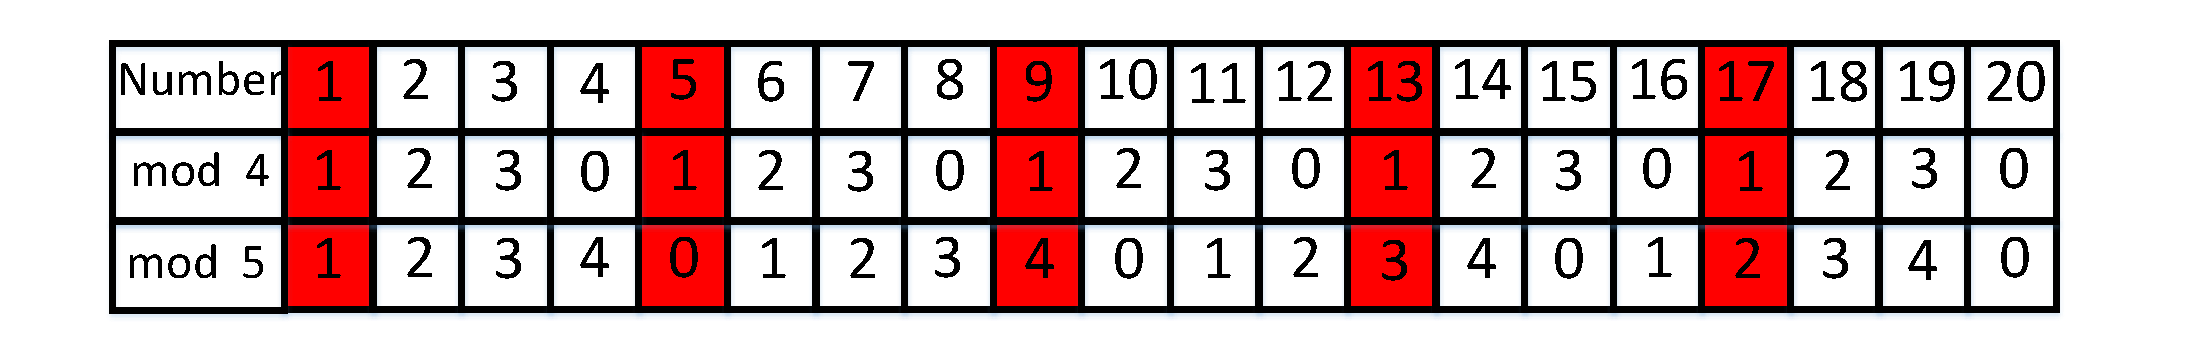
\includegraphics[width=1\columnwidth]{theo}
\caption{An example of Theorem \ref{theo}.}
\label{exp1}
\end{figure}

Fig. \ref{exp1} illustrates an example of Theorem \ref{theo}. In Fig. \ref{exp1}, the first row is a string of numbers starting from 1. The second row is the results of these numbers under modulo 4 arithmetic. The third row is the results of these numbers under modulo 5 arithmetic. We can clearly see that 1, 5, 9, 13, 17 all correspond to 1 under modulo 4 arithmetic, but correspond to 1, 0, 4, 3, 2 respectively under modulo 5 arithmetic, which are all the possible results under modulo 5 arithmetic. Theorem \ref{theo} plays an important role in rendezvous algorithms and is the main tool we use to design the following algorithms.

\subsection{Related Works}
Rendezvous algorithms can be classified into different categories according to different standards. One method is to divide rendezvous algorithms into Global-sequence-based rendezvous algorithms and Local-sequence-based rendezvous algorithms.

\bfseries (i) Global-sequence-based rendezvous algorithms. \mdseries

Global-sequence-based rendezvous algorithms design channel hopping sequence based on all the channels in the network. When a channel is not available to a user, the user replaces it with an arbitrary available channel. Jump-Stay (JS)\cite{Liu2012Jump} algorithm is a representative global-sequence-based algorithm which is composed of two patterns: jump-pattern and stay-pattern. JS algorithm uses the thought of number theory and has an MTTR of $O(n^3)$ where $n$ is the number of channels in the network. Enhanced JS \cite{Lin2013Enhanced}algorithm is an enhanced version of JS algorithm which improves the MTTR to $O(n^2)$ level. Disjoint Relaxed Difference Set (DRDS)\cite{Gu2013Nearly} algorithm is another global-sequence-based rendezvous algorithm. The key of DRDS algorithm is to construct a disjoint relaxed difference set. DRDS algorithm can guarantee rendezvous in $O(n^2)$ timeslots. Channel Rendezvous Sequence (CRSEQ)\cite{Shin2010A} algorithms utilizes the triangle number to generate a channel hopping sequence which also guarantee rendezvous in $O(n^2)$ timeslots.
DSC-based Rendezvous (DSCR)\cite{Yang2016A} algorithm is based on Disjoint Set Cover (DSC), which is an NP-hard problem. DSCR problem generates channel hopping sequences by invoking an approximation construction algorithm of DSC. DSCR algorithm has an MTTR of $(2P+\left \lfloor \frac{P}{2} \right \rfloor)(P-G+1)$ timeslots, where $G$ is the number of common channels that the two users share.

\bfseries (ii) Local-sequence-based algorithms. \mdseries

Local-sequence-based algorithms generate channel hopping sequences based on the set of available channels of a user. Heterogeneous Hopping (HH)\cite{Shin2010A} algorithm is a representative local-sequence-based rendezvous algorithm which is composed of three subsequences named fixed, rotating and parity sequence respectively. HH algorithm uses the thought of number theory and has an MTTR of $O(|C_a||C_a|)$ where $|C_a|$ and $|C_b|$ denotes the sizes  of the sets of continuous sensible channels of user $a$ and $b$ respectively.  Interlocking Channel Hopping (ICH)\cite{Wu2013On} algorithm is based on HH algorithm and takes the congestion problem into consideration. Conversion Based Hopping (CBH)\cite{Gu2014Fully} algorithm is a local-sequence-based rendezvous algorithm which utilizes user' ID. CBH algorithm is also applicable in oblivious scenarios. CBH algorithm has an MTTR of $2l_p$max$\{P_i^2,P_j^2\}$ where $l_p$ is determined by the IDs of user $i$,$j$ and $P_i$,$P_j$ are the smallest  primes which is not less than the sizes of available channel sets of user $i$ and $j$ respectively. A-HCH \cite{Chen2014A} algorithm is another local-sequence-based rendezvous algorithm which utilizes ID. Adv.rdv algorithm constructs channel hopping sequences by generating slow and fast channel hopping sequences and interleaving them. Adv.rdv algorithm has three versions, which are Adv.rdv-Optimal \cite{Chen2014A}, Adv.rdv-$\eta_1$ \cite{Chen2014A} and Adv.rdv-$\eta_2$ \cite{Chen2014A}. The difference of them is the construction of symmetrization classes. Adv.rdv-Optimal is a centralized algorithm which is not applicable to distributed system. Moving Traversing Pointers (MTP) \cite{Gu2015Improved}algorithm utilizes two pointers to generate channel hopping sequences and can guarantee rendezvous in $2(max\{|V_i|,|V_j|\})^2\times32(\left \lceil loglog n\right \rceil +1)$ timeslots.

\section{Model and Problem Formulations}
In this section, we will introduce the foundation model and some other models which are based on the foundation model. Models are of great importance in the design of rendezvous algorithms, because models constrain the resources that we can use. Hence, we need to design different algorithms under different models to achieve high performance for rendezvous process. We will also give the formulation for rendezvous problem in this section.


\subsection{Foundation Model}
 Suppose the licensed spectrum is divided into $n$ channels which are non-overlapping. Denote the set of channels as $U=\{1,2,\cdots,n\}$, where $n$ is the total number of channels in $U$. We assume that every user in the network is equipped with a CRN. User i has a set of available channels as $V_i = \{v_{i1},v_{i2},\cdots,v_{im_i}\}$, where $m_i$ is the number of channels in set $V_i$. For simplicity, we suppose that $V_i$ doesn't change during the rendezvous process. Let the length of every timeslot be 2t, where $t=10ms$ according to IEEE 802.22.

\begin{figure}
\centering
\subfigure[case 1]{
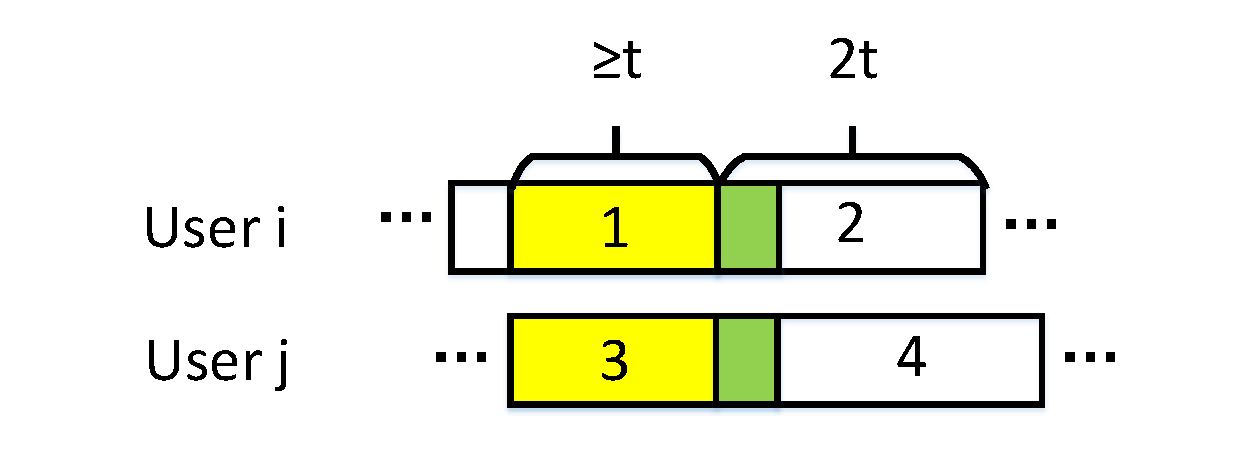
\includegraphics[width=1.6in]{olp1}
\label{olp1}
}
\subfigure[case 2]{
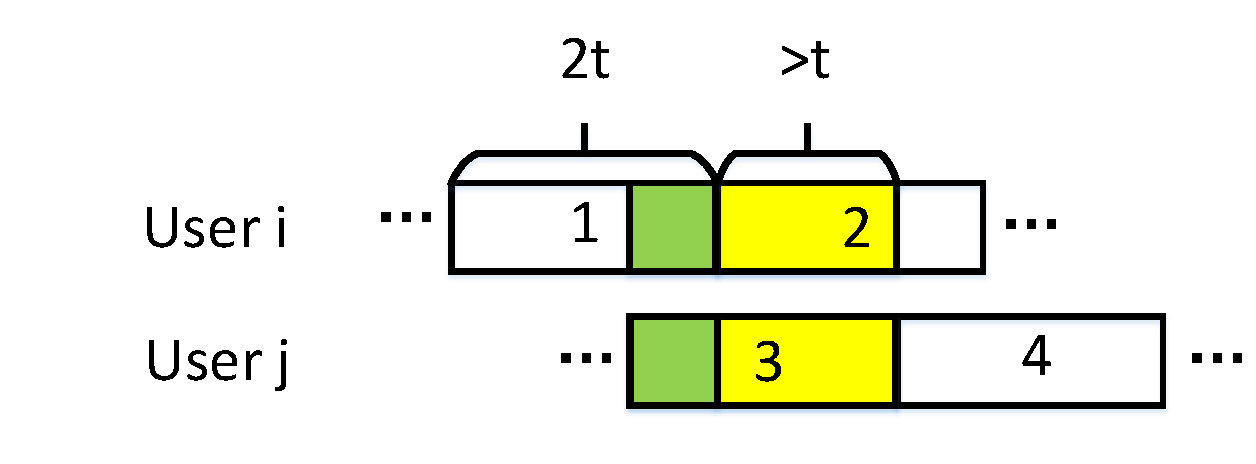
\includegraphics[width=1.6in]{olp2}
\label{olp2}
}
\caption{An example of different cases of timeslot overlapping.}
\label{overlap}
\end{figure}

Because the lengths of all users' timeslots are equal, user j's one timeslot can overlap with at most two consecutive timeslots of user i. Fig. \ref{overlap} illustrates this problem in two cases. Suppose timeslot 3 is one timeslot of user j. And the left timeslot of user i which overlaps with timeslot 3 is timeslot 1. The right timeslot of user i which overlaps with timeslot 3 is timeslot 4. The yellow part stands for the overlapping part of timeslot 1 and 3, while the green part stands for the overlapping part of timeslot 2 and 3. In Fig. \ref{olp1}, the length of the yellow part is greater than or equal to t. In Fig. \ref{olp2}, the length of the green part is greater than t.
There is a special case that the length of the yellow part or the green part is zero, which means that the timeslots of user i and user j are aligned.
Hence, no matter when the users start their rendezvous process, the maximum overlap of their timeslots is at least t, which is enough for two users to find each other and exchange information.Foundation model is the basis of other models we will introduce in the following subsections.
%
%\subsection{Oblivious and Non-Oblivious Models}
%The difference between oblivious and non-oblivious models is whether there exists a global label for every channel in $U$ and users label channels as same as their global labels. In oblivious model, there doesn't exist any global label and every user labels channels in its own way. For example, for the same channel, denote it as c, user i can label it as 1 while user j can label it as 2. In non-oblivious model, there exist global labels for channels such as $U=\{1,2,\cdots,n\}$ where we label the i-th channel in U as i. And the label of every channel for every user is as same as its global label.  It is obvious that designing rendezvous algorithms for oblivious model is at least not easier than non-oblivious model, since in non-oblivious model, we could use the labels of channels as an extra resource for designing rendezvous algorithms.

%\subsection{Anonymous and Non-Anonymous Models}
%The difference between an is whether each user in the network has a unique ID. In anonymous model, there doesn't exist a unique ID for each user. Hence, a user can't be distinguished from the other users. In non-anonymous model, there exists a unique ID for each user. Hence, a user is easily distinguishable from the other users. Designing rendezvous algorithms for non-anonymous model is easier than anonymous model, because we can use IDs, which will be shown very powerful for rendezvous process.
%
%\subsection{Synchronous, Asynchronous and Semi-Synchronous Models}
%In the previous works, there exist synchronous and asynchronous rendezvous algorithms. In synchronous model, there exists a global clock, and time is divided into equal timeslots. And every user start their rendezvous process from the same timeslot. In asynchronous model, there doesn't exist any global clock, time is divided into equal timeslots according to their local clock. And every user can start its own rendezvous process at any time.
%
%In this paper, we introduce a new model about timing, which is semi-synchronous model. In semi-synchronous model, there exists a global clock, and time is divided into equal timeslots. However, every user can start its own rendezvous process at any timeslot. Though synchronous model is difficult to implement, semi-synchronous model is practical. There exist many techniques to achieve time giving, such as GPS timing, Beidou satellite time giving, CSAO time giving and so on. These time services have high precision. For example, GPS timing can achieve 10 nanosecond level precision. Because our timeslot is 20 ms long, this level of precision is enough for our use.
%
%We need to point out that different models in different subsections can be combined to generate a new model. We will propose some algorithms for three combined models.

\subsection{Problem Formulations}
In this paper, we focus on designing rendezvous algorithms for two-user scenario, because it is the fundamental process for multiple-user rendezvous. Two-user rendezvous algorithms can be expanded into multiple-user rendezvous algorithms. Then we give the formulations of the three problems we will solve:
\begin{problem}
Utilize an arbitrary available channel of a user to design an asynchronous anonymous non-oblivious global-sequence-based rendezvous algorithm with low MTTR.
\end{problem}

\begin{problem}
Utilize the ID of a user to design an asynchronous non-anonymous oblivious local-sequence-based rendezvous algorithm with low MTTR.
\end{problem}

\begin{problem}
Utilize an arbitrary available channel of a user to design an asynchronous anonymous non-oblivious local-sequence-based rendezvous algorithm with low  MTTR.
\end{problem}

\section{Sequence-Rotating Rendezvous Algorithm}

In this section, we will propose a global-sequence-based rendezvous algorithm which is based on the channel label.

We first propose an algorithm to generate the subsequences to be used.

\begin{algorithm}
\caption{Subsequence Generating Algorithm}
\label{alg2}
\begin{algorithmic}[1]
\STATE Input: the set of available channels $V=\{v_1,v_2,\cdots,v_m\}$, and length $L$;
\STATE Initialize array $S$ with length $L$;
\STATE Initialize $i :=0$;
\WHILE {$i < L$}
\IF{$i \le m$}
\STATE $S[i] := v_i$;
\ELSE
\STATE Randomly choose a channel from $V$, denote it as $c$;
\STATE $S[i] := c$;
\ENDIF
\STATE $i:=i+1;$
\ENDWHILE
\STATE Output: Sequence $S$.
\end{algorithmic}
\end{algorithm}

The main idea of Alg.\ref{alg2} is to generate a subsequence $S$ with length $L$ according to $V$. The process is rather simple. We fill the first $m$ elements in $S$ with the channels in $V$. For the rest $(L-m)$ elements, we randomly pick channels from $V$ to fill them.


\begin{algorithm}
\caption{Sequence-Rotating Rendezvous Algorithm}
\label{alg1}
\begin{algorithmic}[1]
\STATE Input: the set of available channels $V=\{v_1, v_2, \cdots, v_m\}$ and the total number $N$ of all channels;
\STATE Find the least prime $P$ that ensure $P \ge N$;
\STATE Randomly choose a channel from $V$, denote it as channel ($c$);
\STATE Initialize $t := 0$;
\WHILE {$0 \le t < 2P$}
\STATE Access channel ($c$);
\STATE $t:=t+1$;
\ENDWHILE
\STATE Invoke Alg.\ref{alg2} to generate a subsequence $S$ with channel set $V$ and length $P$;
\WHILE {Not rendezvous}
\IF{$t \ne 2P$ and $t $ mod $ (2P) = 0$}
\STATE Rotate $S$ to the right by $c$ steps;
\ENDIF
\STATE Access channel $S[t$ mod $P]$;
\STATE $t := t + 1$
\ENDWHILE

\end{algorithmic}
\end{algorithm}




In Alg. \ref{alg1}, we first find the least prime which is not less than the total number of  all channels. Then we randomly choose a channel from $V$, denote it as channel ($c$), and access this channel for the first $2P$ timeslots. We call this the \bfseries first stage \mdseries, the following is the \bfseries second stage \mdseries.

Then, we will generate a subsequence $S$ with length $P$. If channel $(a)$ is in the available channel set $V$, the $a-th$ channel in $S$ is channel $(a)$. For the channels that are not exist in $V$, their places will be replaced by channels which are randomly picked from $V$. And the last $(P-n)$ channels in $S$ are randomly picked from $V$. The period is $2P$ timeslots. Then we will rotate the sequence by $c$ steps to the right every period. In every period, we will hop to channels according to rotated sequence.

Fig.\ref{seq1} illustrates an example of the original generated subsequence and the first rotated subsequence. In this example, $V =\{1,3,5,6\}$ and $n=6$, so $P=7$. We generate a sequence as Fig.\ref{sq1}, where the blue rectangles correspond to randomly picked channels. And a rectangle with number in it, denote it as $i$,  represents the Channel ($i$). Because the least label in $V$ is 1, so the sequence is rotated by 1 step to the right every period. The first rotated sequence is shown in Fig.\ref{sq2}.

\begin{figure}
\centering
\subfigure[Original subsequence]{
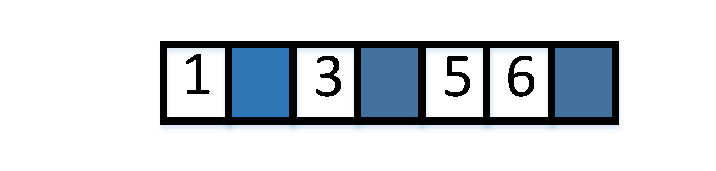
\includegraphics[width=1.6in]{sq1}
\label{sq1}
}
\subfigure[The first rotated subsequence]{

\includegraphics[width=1.6in]{sq2}
\label{sq2}
}
\caption{An example of generated subsequence when $V=\{1,3,5,6\}$, $N=6$ and the first rotated subsequence.}
\label{seq1}
\end{figure}


We then introduce a theorem which will be used in the later discuss.

\begin{theorem}
\label{ro-theo}
Suppose there are two aligned subsequences $S_1$ and $S_2$ with identical length $P$ and $P$ is a prime. Suppose $0 \le k_1 \le P, 0 \le k_2 \le P$ and $k_1 \ne k_2$. If in every period we rotate $S_1$ and $S_2$ to the right by $k_1$ and $k_2$ steps respectively and concatenate them to $S_1$ and $S_2$ respectively. Then after $P$ periods, every element of $S_1$ will meet every element of $S_2$ and vice versa.
\end{theorem}

\begin{figure}[!t]
\centering
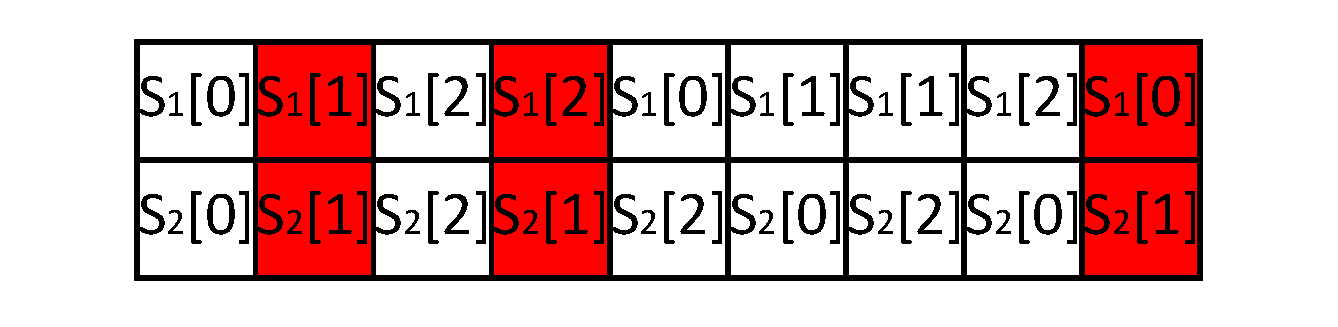
\includegraphics[width=1\columnwidth]{rotate-theo}
\caption{An example of Theorem {\ref{ro-theo}}.}
\label{exp-rotheo}
\end{figure}

\begin{IEEEproof}
Because $S_1$ and $S_2$ are aligned, then $S_1[i]$ will meet $S_2[i]$ in the first period, where $0 \le i < P$. Without lose of generality, suppose $k_1 > k_2$. Let $k_1 - k_2 = m$, then in the later $(P-1)$ periods, $S_1[i]$ will meet $S_2[(i + m)$ mod $P]$, $S_2[(i + 2m)$ mod $P]$, $\cdots$, $S_2[(i+(P-1)m)$ mod $P]$ respectively. According to Theorem \ref{theo}, $i, i + m, i + 2m, \cdots, i + (P-1)m$ are $P$ distinct numbers under modulo-P arithmetic.  Hence, $S_1[i]$ meets all the elements of $S_2$ in $P$ periods and Theorem \ref{ro-theo} holds.
\end{IEEEproof}
Fig.\ref{exp-rotheo} illustrates an example of Theorem {\ref{ro-theo}}, where the length of $S_1$ and $S_2$ is $3$. $S_1$ is rotated to the right by $1$ steps every period, and $S_2$ is rotated to the right by $2$ steps every period. We can clearly see that $S_2[1]$ meets $S_1[1],S_1[2],S_1[0]$ in the three consecutive periods.

\begin{theorem}
\label{theo-alg1}
The MTTR of Alg.\ref{alg1} is $2P^2 + 2P$.
\end{theorem}

\begin{IEEEproof}
We show discuss this problem in two cases.

\bfseries Case 1 \mdseries: Suppose two users choose the same channel, denote it as channel $c$. Without loss of generality, suppose user $i$ starts rendezvous process earlier than user $j$. For clarity, we divide this case into two subcases.

\bfseries Subcase 1.1 \mdseries: Suppose user $j$ starts rendezvous process when user $i$ is still in the first stage, they will both access channel $c$ at the same time. Hence, rendezvous is achieved.

\bfseries Subcase 1.2 \mdseries: Suppose user $j$ starts rendezvous process when user $i$ is already in the second stage. Then in the following $2P$ timeslots, user $i$ will access each available channel including channel $c$ at least once, while user $j$ will stay on channel $c$ in the $2P$ timeslots. Hence, rendezvous can be achieved in the $2P$ timeslots.

\bfseries Case2 \mdseries: Suppose user $i$ and $j$ choose different channels, denote them as channel $(c_i)$ and channel $(c_j)$. When user $i$ and $j$ both get into the second stage, they will both rotate their sequences according to it. There are two situations of periods overlapping of user $i$ and $j$, we will discuss them separately.

\bfseries Subcase 2.1 \mdseries: Suppose the periods of user $i$ and $j$ are aligned, then the scenario is the same as the setting in Theoren \ref{theo} except for that we duplicate the current subsequences before rotate it and attach them to the corresponding sequences. The difference result in double time delay. According to Theorem \ref{ro-theo}, rendezvous will be achieved in $2P^2 + 2P$ timeslots.

\bfseries Subcase 2.2 \mdseries: Suppose the periods of user $i$ and $j$ are not aligned. There are two situations of periods overlapping of user $i$ and $j$ as illustrated in Fig.\ref{sit_period}. The yellow rectangle in Fig.\ref{st1} represents the first half of user $j$'s period, while the red rectangle represents the corresponding part in user $i$'s period. The red rectangle includes all the elements of subsequence $S_i$, because the two halves of user $i$'s period are the same rotated subsequence of $S_i$. Then this situation is similar to Subcase 2.1, and according to Theorem \ref{ro-theo}, rendezvous will be achieved in $2P^2 + 2P$ timeslots. Situation 2 can be analysed in the same way, so we omit it here.

\begin{figure}
\centering
\subfigure[Situation 1]{
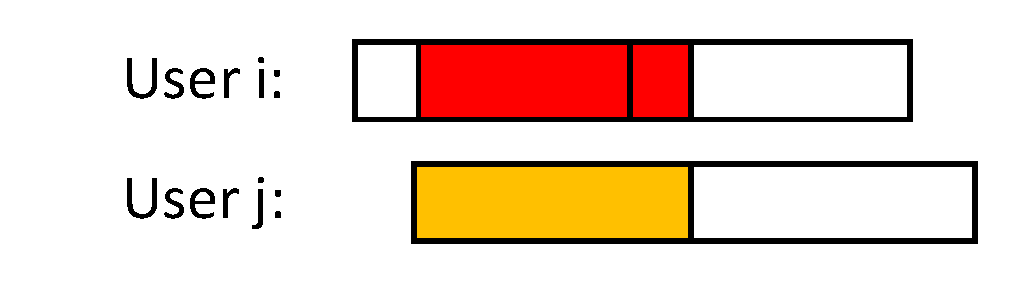
\includegraphics[width=1.6in]{subcasei}
\label{st1}
}
\subfigure[Situation 2]{
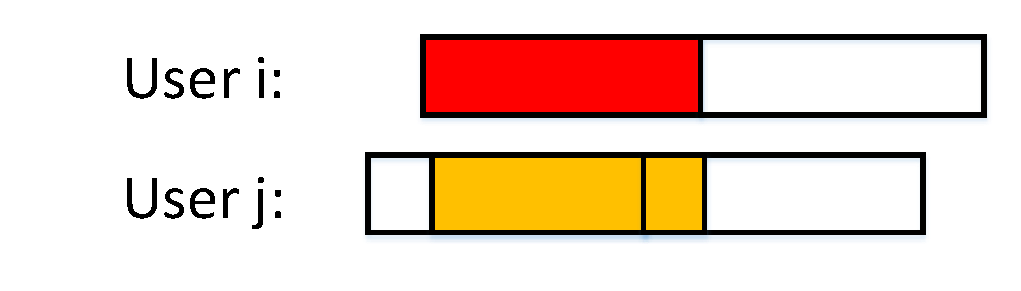
\includegraphics[width=1.6in]{subcaseii}
\label{st2}
}
\caption{Two situations of periods overlapping of user $i$ and $j$}
\label{sit_period}
\end{figure}

Combine these together, we have shown that Theorem \ref{theo-alg1} holds.
\end{IEEEproof}

\section{ID-based Rendezvous Algorithm}
In this section, we will propose an ID-based asynchronous non-anonymous oblivious rendezvous algorithm. The main idea of this algorithm is to create a channel hopping sequence composed of $(l + 1)$ subsequences, where $l$ is the length of ID.

\begin{algorithm}
\caption{Local-sequence-based Non-Anonymous Rendezvous Algorithm}
\label{alg3}
\begin{algorithmic}[1]
\STATE Input: the set of available channels $V=\{v_1,v_2,\cdots,v_m\}$, and its binary ID whose length is $l$ bits;
\STATE Find the smallest prime $P$ that ensure $P \ge m$;
\IF{$P = 3$}
\STATE $P:= 5$;
\ENDIF
\STATE Initialize $t := 0, i:= 0, j:= 0$;
\STATE Invoke Alg.\ref{alg2} to generate three sequences $S_1,S_2,S_3$ with channel set V and length $P, P+1, P+2$ respectively;
\STATE Find the channel with the least label in $V$, denote it as channel $(c)$;

\WHILE{Not rendezvous}
\STATE $i := \left \lfloor t / (l+1) \right \rfloor$;
\STATE $j := t $ mod $(l  +1)$;
\IF{$ j < l$}

  \IF{ID$[j] = 0$}
   \STATE Access channel $S_2[i$ mod $(P+1)]$;
    \ELSE
    \STATE Access channel $S_3[i$ mod $ (P+2)]$;
    \ENDIF
\ELSE
\STATE Access channel $S_1[i $ mod $ P]$;
\ENDIF
\STATE $t := t + 1$;
\ENDWHILE

\end{algorithmic}
\end{algorithm}


In Alg.\ref{alg3}, we creates a channel hopping sequence consisting of $(l +1)$ subsequences. The $(l +1)$ subsequences are generated by Alg.\ref{alg2}. There are three kinds of subsequences, which are $S_1, S_2$ and $S_3$. The lengths of $S_1, S_2$ and $S_3$ are P, P+1, P+2 respectively.

Fig.\ref{exp-alg3} illustrates an example of Alg.\ref{alg3}. In this example, the length of ID is 5 and user i's ID is 01101. In round 1, the first $ l$ elements of round 1 are either $S_2[0]$ or $S_3[0]$. If the corresponding digit of the i-th element in ID is 0, then the i-th element will be $S_2[0]$. If the corresponding digit of the i-th element in ID is 1, then the i-th element will be $S_3[1]$. The last element of round 1 is $S_1[0]$.

\begin{theorem}
\label{theo-alg3}
Alg.\ref{alg3} can guarantee rendezvous for two asynchronous users in $(l  + 1)(P_i + 2)(P_j + 2)$ timeslots if $V_i \cap V_j \ne \emptyset$.
\end{theorem}

\begin{figure}[!t]
\centering
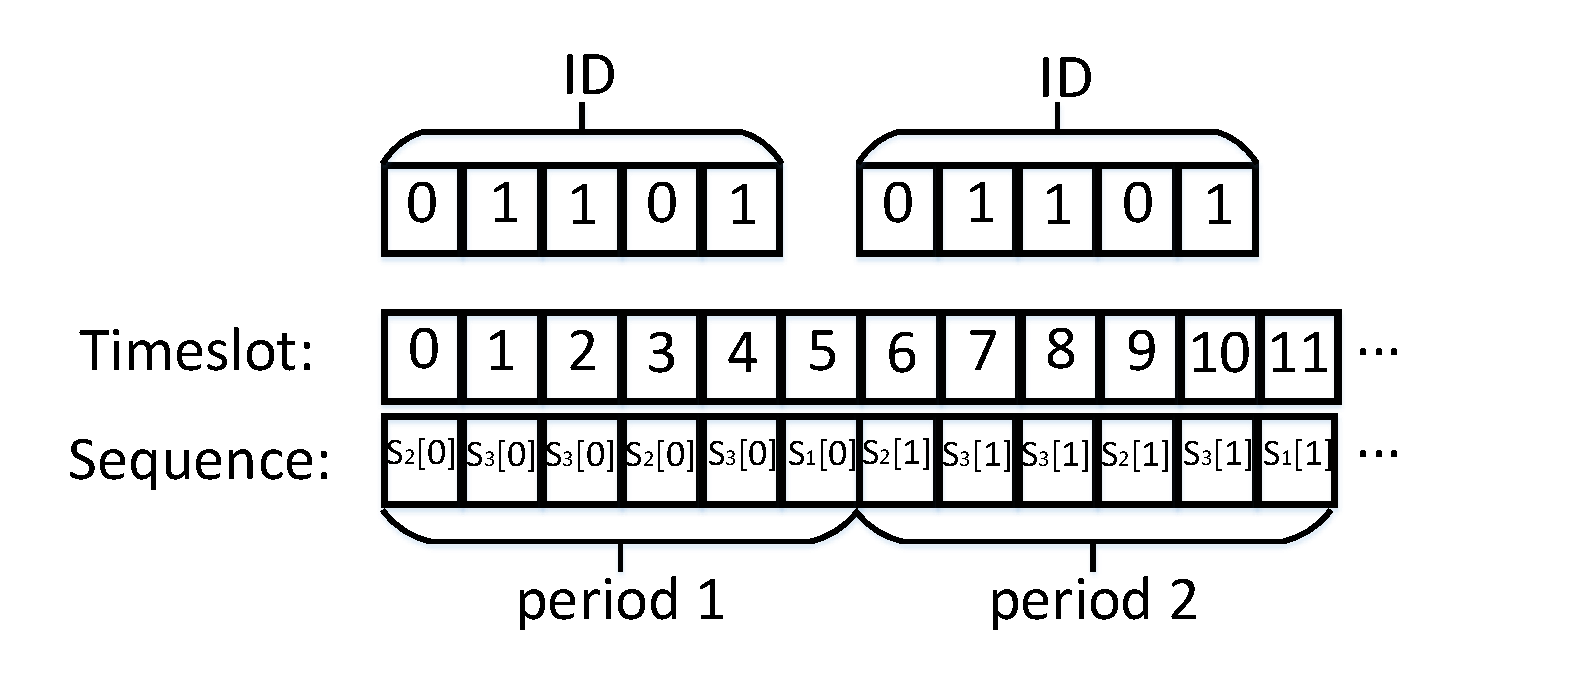
\includegraphics[width=1\columnwidth]{round}
\caption{An example of Alg. {\ref{alg3}}.}
\label{exp-alg3}
\end{figure}


\begin{figure}
\centering
\subfigure[subcase 1]{
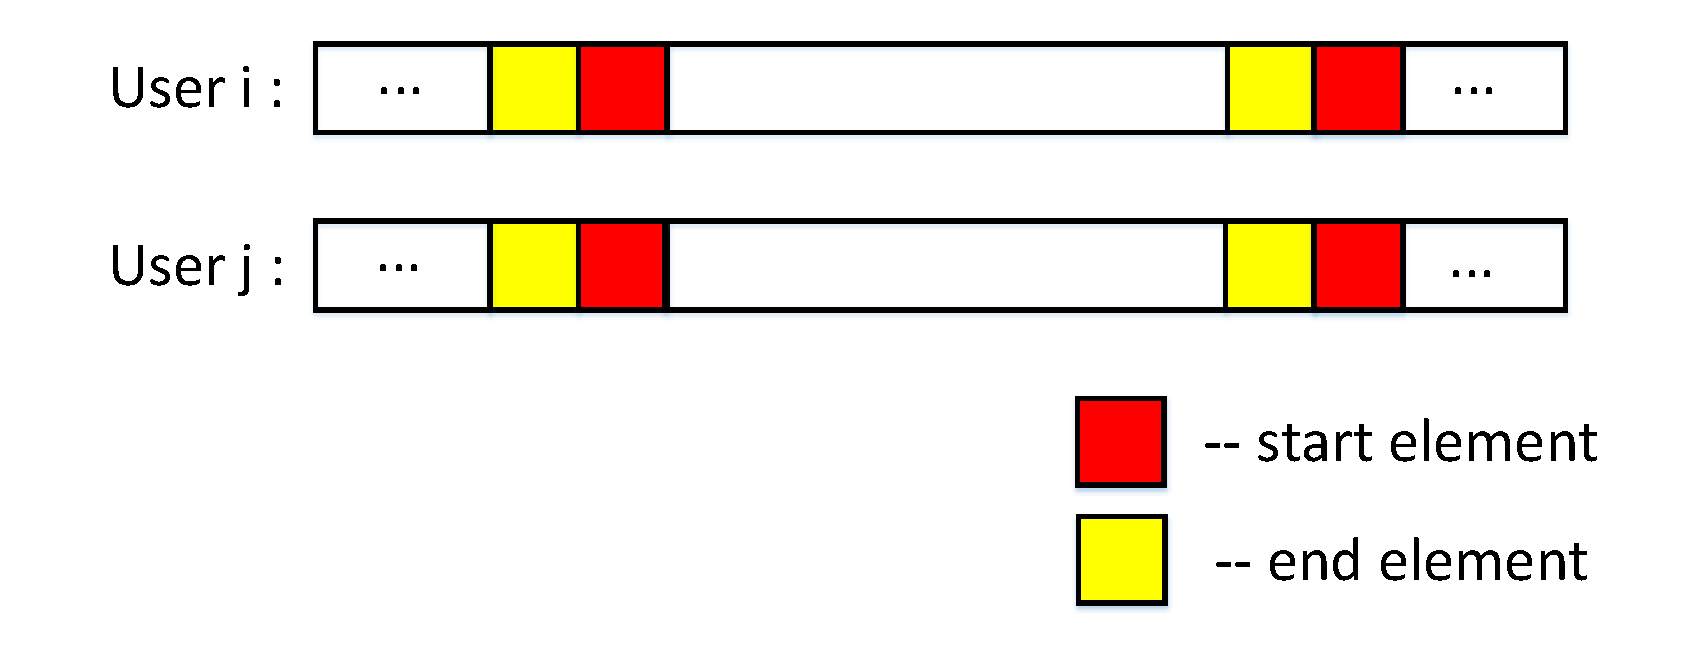
\includegraphics[width=1.6in]{case1}
\label{cs1}
}
\subfigure[subcase 2]{
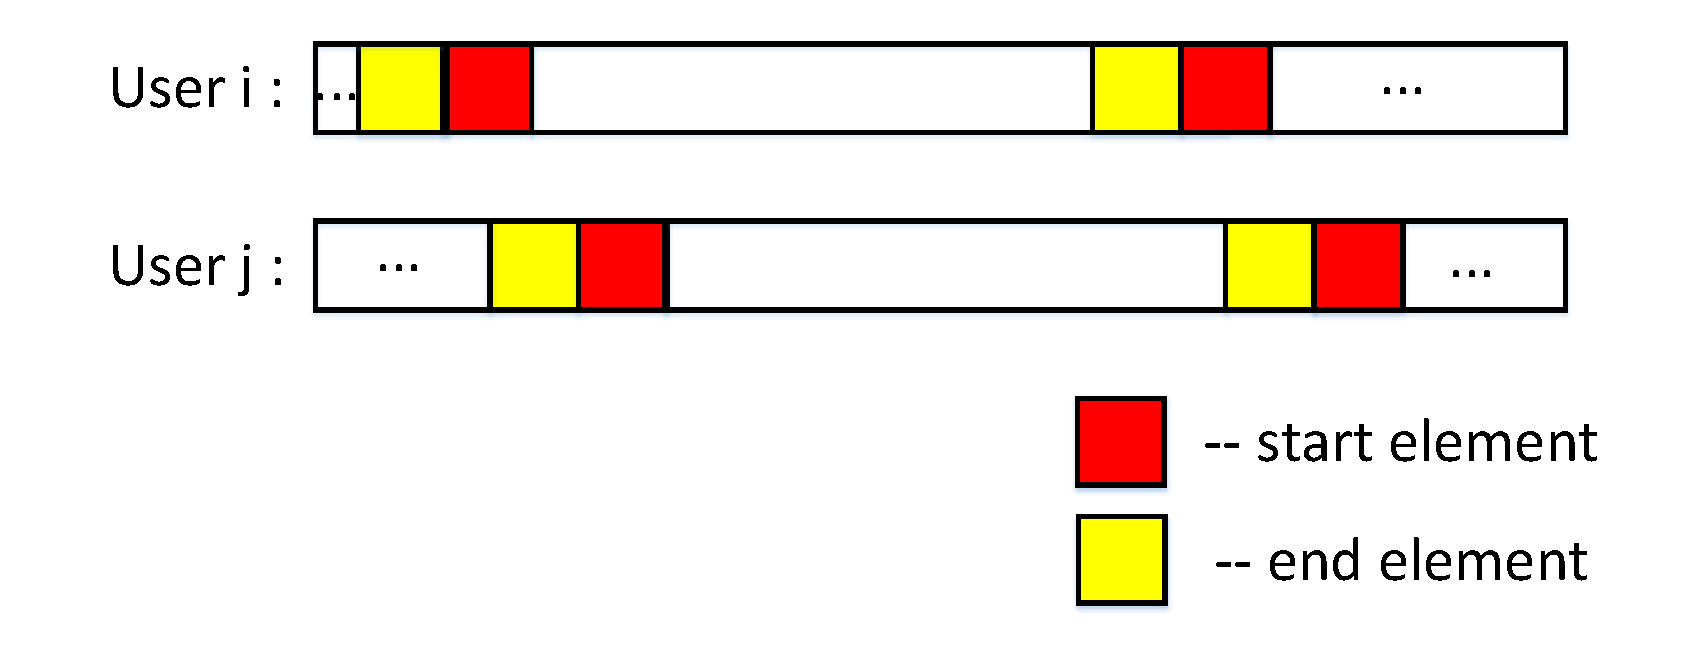
\includegraphics[width=1.6in]{case2}
\label{cs2}
}
\caption{Two subcases of case 1 and case 2.}
\label{case}
\end{figure}



\begin{IEEEproof}
We discuss in two cases:

\bfseries Case 1 \mdseries:

 Suppose $P_i = P_j$. Let $P = P_i =P_j$ We divide this case into two subcases:

\bfseries Subcase 1.1 \mdseries: Suppose user i and j's periods are aligned, as illustrated in Fig.\ref{cs1}. Because user i and user j are two different users, their ID must be different in at least one digit. Without lose of generality, suppose the k-th digit in $ID_i$ is 0 while the k-th digit in $ID_j$ is 1. Then the k-th element in user i's period corresponds to subsequence $S_{2i}$, whose length is $P+1$. The k-th element in user j's period corresponds to subsequence $S_{3j}$, whose length is $P+2$. Then in every period, one element of $S_{2i}$ will meet one element of $S_{2j}$. According to Lemma \ref{lm2.3}, P+1 and P+2 are co-prime. Then rendezvous can be achieved in $(l+ 1)(P+1)(P+2)$ timeslots according to Theorem \ref{theo}, as long as user i and j have at least one common channel.

\bfseries Subcase 1.2 \mdseries: Suppose user i and j's periods are not aligned, as illustrated in Fig.\ref{cs2}. In this case, the last element in user i's period will meet one of the first $(l + 1)$ elements of user j's period. The last element in user i's period corresponds to subsequence $S_{1i}$. The corresponding element of user j corresponds to subsequence $S_{2j}$ or $S_{3j}$. From Lemma \ref{lm2.3} and \ref{lm2.4}, we know that P and P+1 are co-prome, P and P +2 are also co-prime. Hence, according to Theorem \ref{theo}, rendezvous can be achieved in $(l + 1)P(P+1)$ or $(l + 1)P(P+2)$ timeslots respectively.

\bfseries Case 2 \mdseries: Suppose $P_i \ne P_j$.  We divide this case into two subcases:

\bfseries Subcase 2.1 \mdseries: Suppose user i and j's periods are aligned, as illustrated in Fig.\ref{cs1}. In this case, the last
element in user i's period will meet the last element in user j's period. The last element in user i's period corresponds to subsequence $S_{i1}$. The last element in user j's period corresponds to subsequence $S_{j1}$. Because $P_i \ne P_j$, rendezvous can be achieved in $(l + 1)P_iP_j$ timeslots according to Theorem \ref{theo}, as long as user i and j have at least one common channel.

\bfseries Subcase 2.2 \mdseries: Suppose user i and j's periods are not aligned, as illustrated in Fig.\ref{cs2}. Without lose of generality, suppose $P_i > P_j$. In this case, the last element in user i's period will meet one of the first $(l + 1)$ elements of user j's period. The last element in user j's period will meet one of the first $(l + 1)$ elements of user i's period. The last element in user j's period corresponds to subsequence $S_{1j}$, whose length is $P_j$. The corresponding element of user j corresponds to subsequence $S_{2i}$ or $S_{3i}$, whose lengths are $P_i +1$ and $P_i +2$ respectively. Because $P_i$ and $P_j$ are two different primes, $P_i > P_j +2$ or $P_i = P_j +2$. If $P_i > P_j + 2$, from Lemma \ref{lm2.5}, we know $P_i$ and $P_j + 1$ are co-prime, $P_i$ and $P_j +2 $ are co-prime. According to Theorem 2, rendezvous can be achieved in $(l + 1)P_i(P_j+1)$ or $(l + 1)P_i(P_j+2)$ timeslots respectively. If $P_i = P_j + 2$, then $P_i + 1 = P_2 + 3$, $P_i + 2 = P_j + 4$. If $P_j = 2$, $P_i = 2 + 2=4$ is not a prime. In Alg.\ref{alg3}, we set P to be 5 if $P=3$. Because $P_2 \ne 2$ and $P_2 \ne 3$, $P_2 + 3$ and $P_2 + 4$ can not be divided by $P_2$ without remainder. From Lemma \ref{lm2.5}, we know that both $P_i + 1$ and $P_i +2$ are co-prime with $P_j$. According to Theorem \ref{theo}, rendezvous can be achieved in $(l + 1)(P_i + 1)P_j$ or $(l + 1)(P_i+2)P_j$ timeslots respectively.

Combine the above together, Theorem \ref{theo-alg3} holds.

\end{IEEEproof}


\section{Channel-Label-based Rendezvous Algorithm}
In this section, we will propose a Channel-Label-based Rendezvous (CLR) algorithm which utilizes the label of an arbitrary channel in the available channel set.
\begin{algorithm}
\caption{Channel-Label-based Rendezvous Algorithm}
\label{alg4}
\begin{algorithmic}[1]
\STATE Input: the set of available channels $V=\{v_1,v_2,\cdots,v_m\}$ and the number of all channels: $N$;
\STATE Find the smallest prime $P_N$ that ensure $ P_N \ge N$ and $P_N \ge 5$;
\STATE Find the smallest prime $P$ that ensure $P \ge m$ and $P \ge 5$;

\STATE Initialize $l:=\left \lceil log_2 N \right \rceil$;
\STATE Initialize $t := 0$;
\STATE Randomly choose a channel $(c)$ from $V$;
\STATE Convert $c$ into a binary string $CH$ whose length is $l$;

\WHILE{Not rendezvous and $t < (l+1)P_N$}
\STATE Access channel $(c)$;
\ENDWHILE
\STATE Invoke Alg.\ref{alg3} to achieve rendezvous with channel set $V$, binary string $CH$ and length $l$;
\end{algorithmic}
\end{algorithm}

The main idea of Alg.\ref{alg4} is to randomly choose an available channel $c$ from $V$ and use the binary representation of $c$ as the user's ID. It is obvious that the available channel chosen by two users can be identical, but our algorithm can solve this problem, because the label of an available channel is very useful. Alg.\ref{alg4} is composed of two phases, the first phase is the first $(l+2)P_N$ timeslots, the following is the second phase.
In the \bfseries first phase \mdseries, the user stays on the chosen channel $(c)$. In the \bfseries second phase \mdseries, the user invoke Alg.\ref{alg3} to achieve rendezvous with the binary representation of $c$ as ID.



\begin{theorem}
\label{theo-alg4}
Alg. \ref{alg4} can guarantee rendezvous for two asynchronous users $i$ and $j$ in $((P_i +2)(P_j+2)+P_N)(\left \lceil log_2 N \right \rceil + 1)$ timeslots as long as $V_i \cap V_j \ne \emptyset$.
\end{theorem}

\begin{IEEEproof}

We discuss this problem in two cases.

\bfseries Case 1: \mdseries Suppose the channels $c_i$ and $c_j$ chosen by user $i$ and $j$ respectively are different, then the corresponding binary representations of $c_i$ and $c_j$ are different in at least one digit. Therefore, they can replace the roles of IDs for user $i$ and $j$ respectively. Hence, by invoking Alg.\ref{alg3}, rendezvous can be achieved in $((P_i +2)(P_j+2)+P_N)(\left \lceil log_2 N \right \rceil + 1)$ timeslots.

\bfseries Case 2: \mdseries Suppose the channels $c_i$ and $c_j$ chosen by user $i$ and $j$ respectively are the same, let $c = c_i = c_j$. Then channel $(c)$ must be a common channel of user $i$ and $j$. Without lose of generality, suppose user $i$ starts rendezvous process earlier than user $j$. We then divide this case into two subcases.

\bfseries Subcase 2.1 \mdseries Suppose when user $j$ starts rendezvous process, user $i$ is still in the \bfseries first phase \mdseries.
Then user $j$ will hop to channel $(c)$ in its first timeslot and user $i$ is also in channel $(c)$, hence rendezvous is achieve is achieved in $1$ timeslot.

\bfseries Subcase 2.2 \mdseries Suppose when user $j$ starts rendezvous process, user $i$ is already in the \bfseries second phase \mdseries. Because  user $j$ stays on channel $(c)$ for $P_N(\left \lceil log_2 N \right \rceil + 1)$ timeslots, and $P_N \ge P_i$, hence channel $(c)$ will meets every elements of user $i$'s subsequence $S_1$ (defined in Alg.\ref{alg3}). Therefore, rendezvous will be achieved in the \bfseries first phase \mdseries of user $j$.

Combine these together, Theorem \ref{theo-alg4} holds.

\end{IEEEproof}



\section{Simulation}

In this section, we will show the simulation results of comparing  our algorithms  with state-of-the-art algorithms. We implemented the algorithms in C++ language. And for each experiment, we run the corresponding algorithm for $10000$ times.

 We first compare our SRR algorithm with a representative asynchronous non-anonymous non-oblivious global-sequence-based rendezvous algorithm -- DRDS. Denote $R_i$ and $R_j$ as the ratios of $|V_i|$ and $|V_j|$ to $n$ respectively. First, we set $V_i = \{0.3n, 0.3n +1,\cdots, 0.5n\}, V_j =\{0.5n, 0.5n + 1,\cdots, 0.7n -1 \}$ where $n$ is the total number of channels in the network. In this case, $R_i = R_j = 0.3$. We set the number of common channels to be $1$ in order to reduce the impact of the randomly channel hopping in the both algorithms. We increase $n$ from $10$ to $100$ by $10$ steps each time. The result is illustrated in Fig.\ref{result1}, from which we can clearly see that the MTTR of SRR grows slower than that of DRDS.  Then we set $V_i = \{1,2,\cdots, 0.5n\}$ and $V_j = \{0.5n, 0.5n + 1, \cdots, n -1 \}$. In this case, $R_i = R_j = 0.5$. The result is illustrated in Fig. \ref{result2}. We can clearly see that the MTTR of SRR grows slower than that of DRDS. And we can find the ratio of the MTTR of DRDS to that of SRR in Fig.\ref{result1} is larger than that in Fig.\ref{result2} and more close to the theoretical analysis. The reason is the ratio of the number of common channel to the total channel number decreases with the increase of $R_i$ and $R_j$, which makes it harder for user $i$ and $j$ to choose the same channel simultaneously.

\begin{figure}[htbp]
\centering
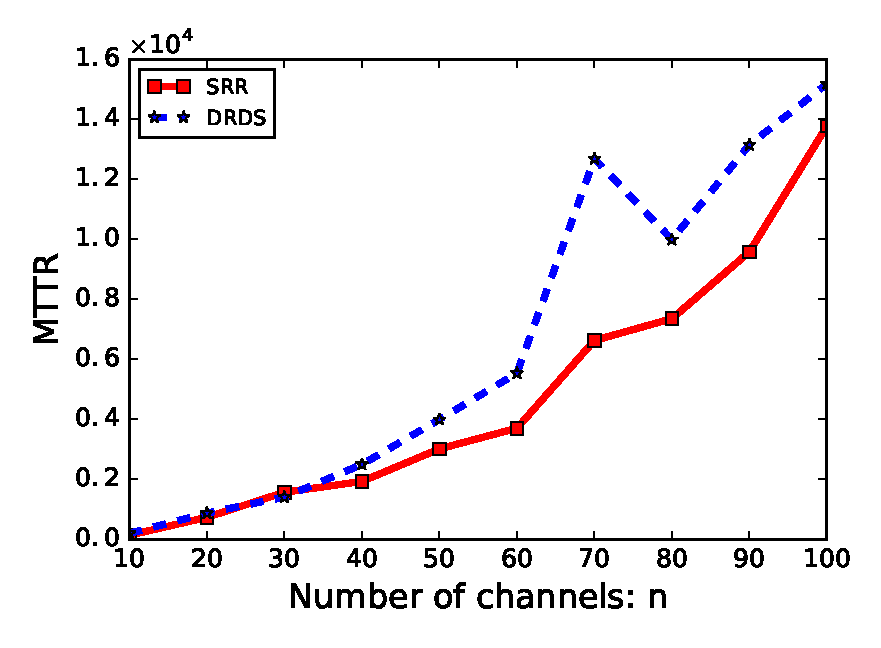
\includegraphics[width=0.7\columnwidth]{fig2}
\caption{Comparison between the SRR algorithm and the DRDS algorithm when $N$ increases from $10$ to $100$ and $R_i = R_j = 0.2$.}
\label{result2}
\end{figure}

\begin{figure}[htbp]
\centering
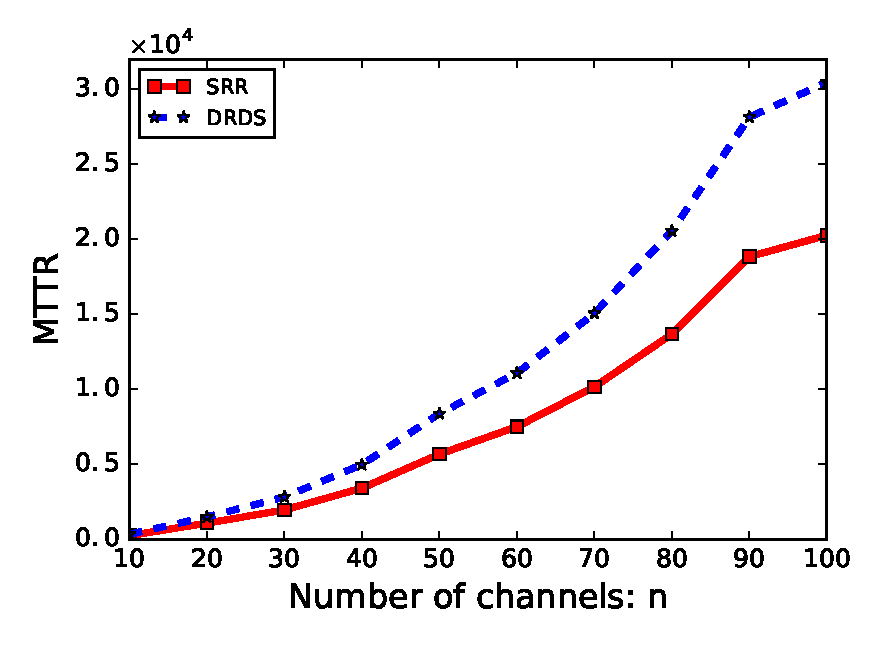
\includegraphics[width=0.7\columnwidth]{fig1}
\caption{Comparison between the SRR algorithm and the DRDS algorithm when $N$ increases from $10$ to $100$ and $R_i =R_j = 0.5$.}
\label{result1}
\end{figure}


\begin{figure}[htbp]
\centering
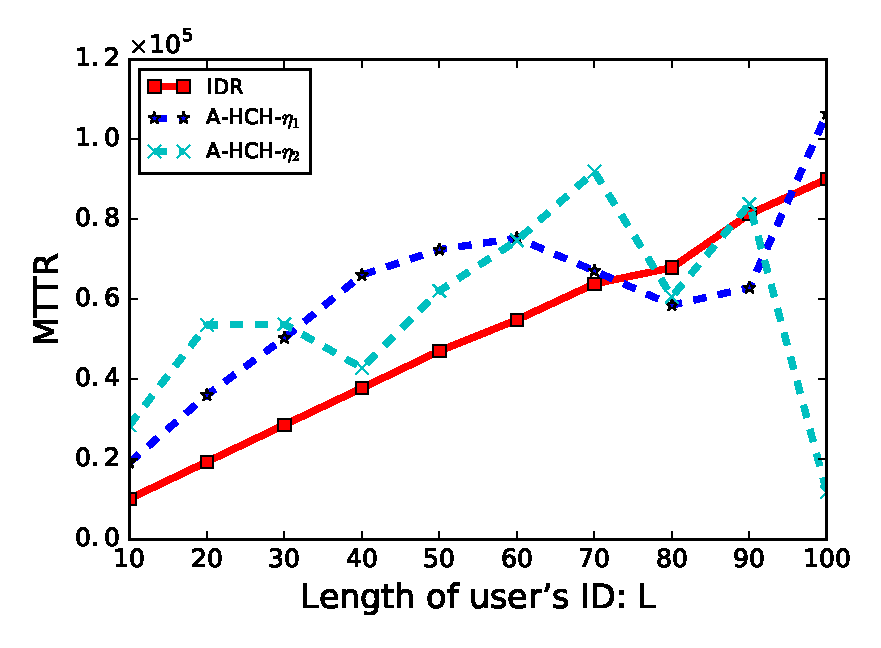
\includegraphics[width=0.7\columnwidth]{fig4}
\caption{Comparison between the IDR algorithm and the A-HCH-$\eta_1$/$\eta_2$ algorithms when $l$ increases from $10$ to $100$ and $N = 50$.}
\label{result4}
\end{figure}

\begin{figure}[htbp]
\centering
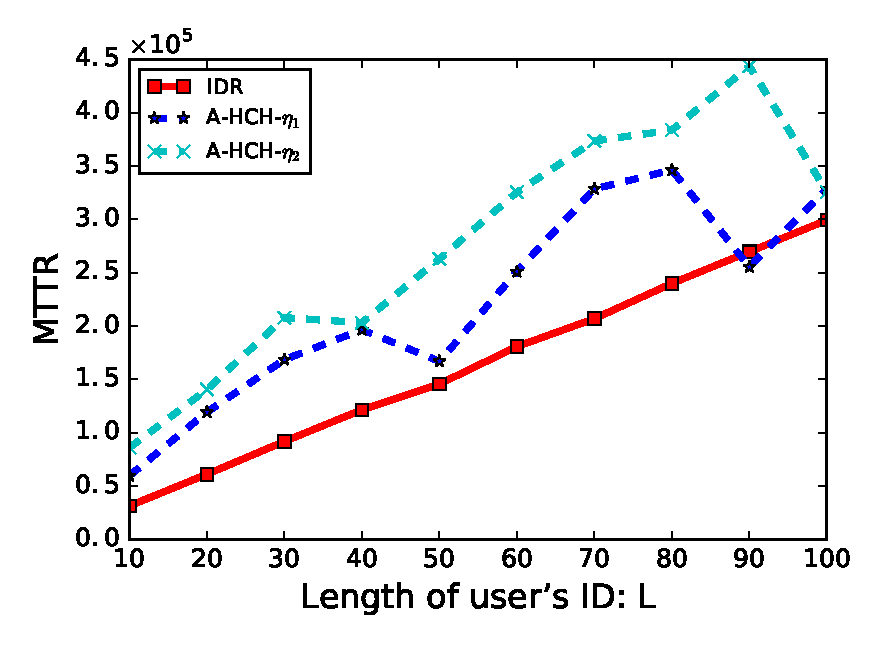
\includegraphics[width=0.7\columnwidth]{fig3}
\caption{Comparison between the IDR algorithm and the A-HCH-$\eta_1$/$\eta_2$ algorithms when $l$ increases from $10$ to $100$ and $N=100$.}
\label{result3}
\end{figure}

\begin{figure}[htbp]
\centering
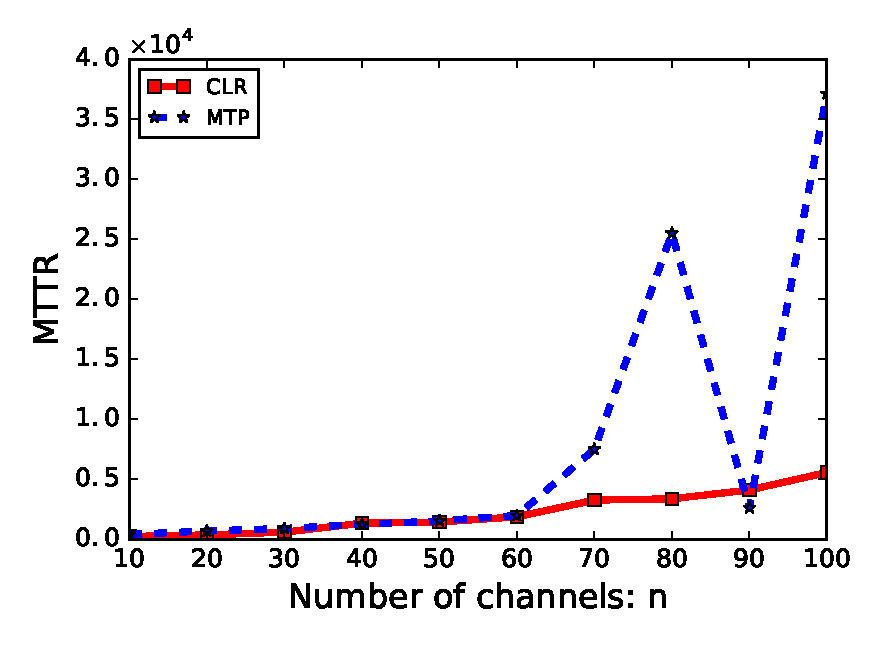
\includegraphics[width=0.7\columnwidth]{fig6}
\caption{Comparison between the CLR algorithm and the MTP algorithm when $N$ increases from $10$ to $100$ and $R_i = R_j = 0.2$.}
\label{result6}
\end{figure}

\begin{figure}[htbp]
\centering
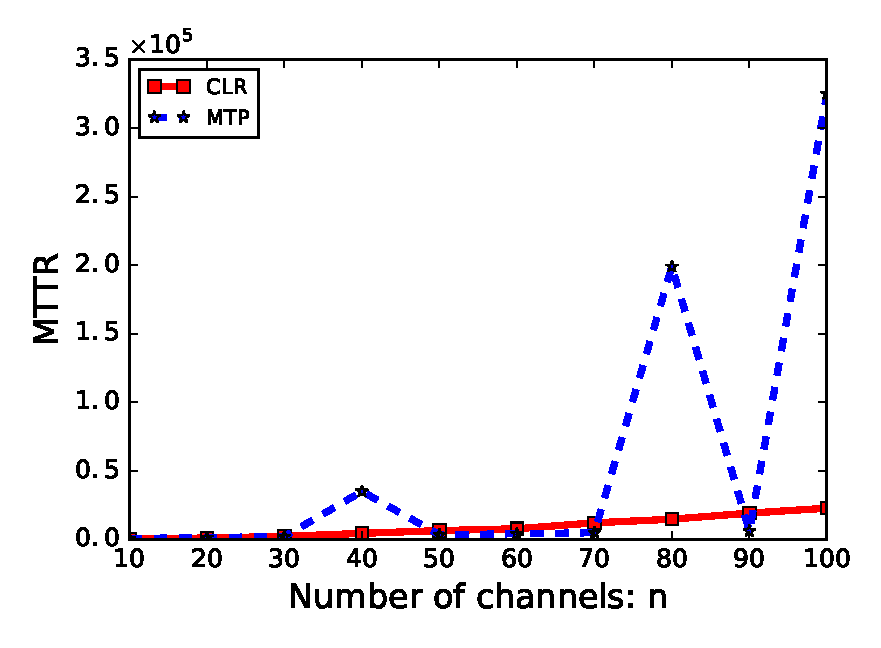
\includegraphics[width=0.7\columnwidth]{fig5}
\caption{Comparison between the CLR algorithm and the MTP algorithm when $N$ increases from $10$ to $100$ and $R_i =R_j = 0.5$.}
\label{result5}
\end{figure}
Second, we conduct experiments to compare the MTTRs of the IDR algorithm and the state-of-the-art asynchronous non-anonymous oblivious local-sequence-based algorithms -- A-HCH-$\eta_1$ and A-HCH-$\eta_2$. For this kind of rendezvous algorithm, the crux is the relationship between the increase of MTTR with the increase of the length of user' ID. Hence, we conduct experiments which fixes $R_i$, $R_j$ and $N$ but increases the length of ID $l$ step by step. We first fix $R_i = R_j = 0.5$ by setting $V_i = \{1,2,\cdots, 0.5n\}$ and $V_j = \{0.5n, 0.5n + 1, \cdots, n -1 \}$. We fix $N = 50$ and increase $l$ from $10$ to $100$ by $10$ steps each time. The result is illustrated in Fig.\ref{result4}. We can clearly see that the MTTR of IDR is less than that of A-HCH-$\eta_1$ or A-HCH-$\eta_2$ in general.
Then we repeats this experiment except for increasing $N$ to $ 100$. The result is illustrated in Fig.\ref{result3}. We can clearly see that the MTTR of IDR is less than that of A-HCH-$\eta_1$ or A-HCH-$\eta_2$ in general.


Third, we implement experiments to compare our CLR algorithm with the state-of-the-art asynchronous anonymous non-oblivious local-sequence-based algorithm -- MTP. MTP has a theoretical MTTR of $O(|V_i||V_j|loglogn)$. We first set $R_i = R_j = 0.2$ by setting $V_i = \{0.3n, 0.3n +1,\cdots, 0.5n\}, V_j =\{0.5n, 0.5n + 1,\cdots, 0.7n -1 \}$. We increase $n$ from $10$ to $100$ by $10$ steps each time. The result is illustrated in Fig.\ref{result6}. We can clearly see that the MTTR of CLR is less than that of MTP in general, and the MTTR of MTP on some experiment points is very large. This is because the MTP algorithm is designed to be relatively complicated in order to achieve MTTR in $O(|V_i||V_j|loglogn)$ order, however, it results in a large constant coefficient. Hence, the MTTR of MTP algorithm can be very high, result in losing superiority. We implement another experiment by increasing $R_i$ and $R_j$ to $0.5$, the result is illustrated in Fig.\ref{result5}. We can see that the situation is similar to that in Fig.\ref{result6}.



\section{Conclusion}
In this paper, we first propose an Sequence-Rotating Rendezvous (SRR) algorithm, which utilizes the label of an arbitrary available channel of a user as local information to generate channel hopping sequence. SRR algorithm uses the thought of number theory and has an MTTR of $(2P^2 + 2P)$ timeslots. Second, we utilize the user's identifier (ID) to design an ID-based Rendezvous (IDR) algorithm. IDR algorithm also uses the thought of number theory and has an MTTR of $(l+1)(P_i+2)(P_j+2)$ timeslots, where $l$ is the length of ID and $P_i$ and $P_j$ are the smallest primes which are not less than the size of available channel sets of user $i$ and $j$ respectively. Third, we propose a Channel-Label-based Rendezvous (CLR) algorithm which can guarantee rendezvous for any two users in $((P_i +2)(P_j+2) + P_N)(\left \lceil log_2 N \right \rceil + 1)$ timeslots, where $N$ is the overall amount of channels in the network and $P_N$ is the least prime which is not less than $N$. CLR algorithm utilizes the binary representation of an arbitrary available channel of a user as the user's ID. CLR algorithm has an MTTR of $((P_i + 2)(P_j + 2) +P_N)(\left \lceil log_2 N \right \rceil + 1)$ timeslots. We conducted plenty of experiments comparing our algorithms with state-of-the-art rendezvous algorithms and the results show our algorithms can achieve good performance.



%
\bibliographystyle{plain}
\bibliography{references}

\end{document}


